\chapter{Vérifications et validations}\label{sec:verif}
\section{Programme de simulation et représentation graphique}
Afin de pouvoir tester l'exécution du procédé et des différentes commandes (du Pacman, du fantôme et des murs), nous avons réalisé un script (\emph{Simulation.m}) qui exécute le procédé commandé sans interface graphique. Il lance l'évolution jusqu'à ce que l'on remplisse une condition d'arrêt (le Pacman est sorti, un objet est bloqué ou le fantôme a attrapé le Pacman). Ensuite, il affiche un compte rendu de l'exécution dans le terminal (nombre d'évolutions et raison de l'arrêt). Puis, il sauvegarde le flux de sorties de toutes les itérations dans un fichier \emph{state.mat} et appelle une fonction qui génère une vidéo et des images afin d'avoir une représentation graphique de l'évolution du labyrinthe. Le tout est stocké dans un dossier nommé en fonction de la date. La fonction de génération de rendu graphique existe en 2 versions. La première est une version basique \emph{CreatePituresAndVideo.m} (figure \ref{fig:4_simu}). La seconde nécessite un lot de textures (qui peuvent être modifiable) \emph{CreatePituresAndVideo\_textured.m} (figure \ref{fig:4_simutext}). % De rien. Bisouss. Lucien

\begin{figure}[!ht]
\begin{minipage}{.48\textwidth}
\centering
\vfill%

\includegraphics[width = .5\textwidth]{./4_Verifications/Simu.jpg}
\caption{\label{fig:4_simu}Image de la première version.}\vfill%
\end{minipage}\hfill%
\begin{minipage}{.48\textwidth}
\centering
\vfill%
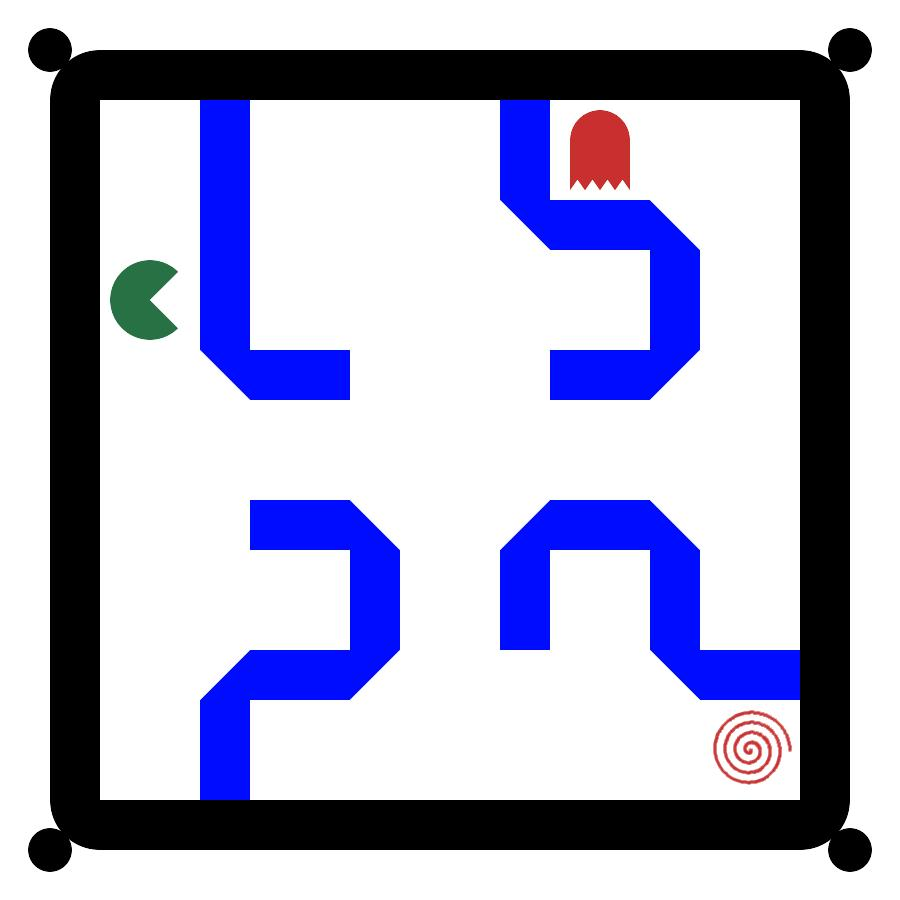
\includegraphics[width = .5\textwidth]{./4_Verifications/Simu_textured.jpg}
\caption{\label{fig:4_simutext}Image de la seconde version.}\vfill%
\end{minipage}
\end{figure}
Il est notable que la seconde version donne un meilleur résultat visuel (c'est celle que nous détaillerons ci-après) mais c'est la première version que nous avons utilisée pour les premiers tests logicielles desquels nous avons issus quelques bugs (voir partie Vérification Logicielle).

\subsection{Script de Visualisation}
Au début de ce script, dans la partie \emph{PARAMETERS}, on a fixé le nombre maximal d'itérations  à $100$.  Il peut être modifié en fonction du besoin. Celui-ci permet de brider la longueur de la simulation pour éviter d'éventuel cas de boucle infinie ou de grande simulation qui impliquerait un gros stockage de données. Ensuite, toujours dans la même partie, sont fixées les conditions initiale du labyrinthe (position initiale des objets, de la sortie et des murs) et des commandes. La seconde partie, \emph{MAIN SCRIPT} commence par la création d'une instance de la classe  \emph{Wrapper} et la connexion de toutes les commandes. Elle contient également une boucle dans laquelle est lancée la simulation jusqu'à ce qu'une des conditions d'arrêt soient satisfaites ou que nous aillons atteint le nombre maximum d'itérations. La fin de cette partie permet de générer le rapport dans le terminal. La dernière partie est l'appel de la fonction de génération de rendu image et vidéo.
\subsection{Fonction de génération d'images et de vidéo}
Comme vu précédemment, la fonction \emph{CreatePituresAndVideo\_textured} utilise un ensemble d'images comme texture et les positionnements de façon à créer une image fidèle de l'état du labyrinthe. Pour cela, nous avons créé 12 images présentées sur la figure \ref{fig:texture}.  Les images correspondent à :
\begin{description}
\item[0] Une case vide.
\item[1] Une case occupée par Pacman.
\item[2] Une case occupée par Ghost.
\item[3] Une case où est la sortie.
\item[4] Une case où Pacman est sur la sortie.
\item[5 à 8 et 23 à 26] Les bordures de l'image.
\item[9 à 12] Les coins des bordures.
\item[13 et 15] L'absence de murs.
\item[14 et 16] Les murs.
\item[17] Les croisements de murs vides.
\item[18] Les croisements de murs pleins.
\item[19 à 22] Les croisements de murs obliques
\end{description}

\begin{figure}[!ht]
\begin{minipage}{.48\textwidth}
\centering
\vfill%
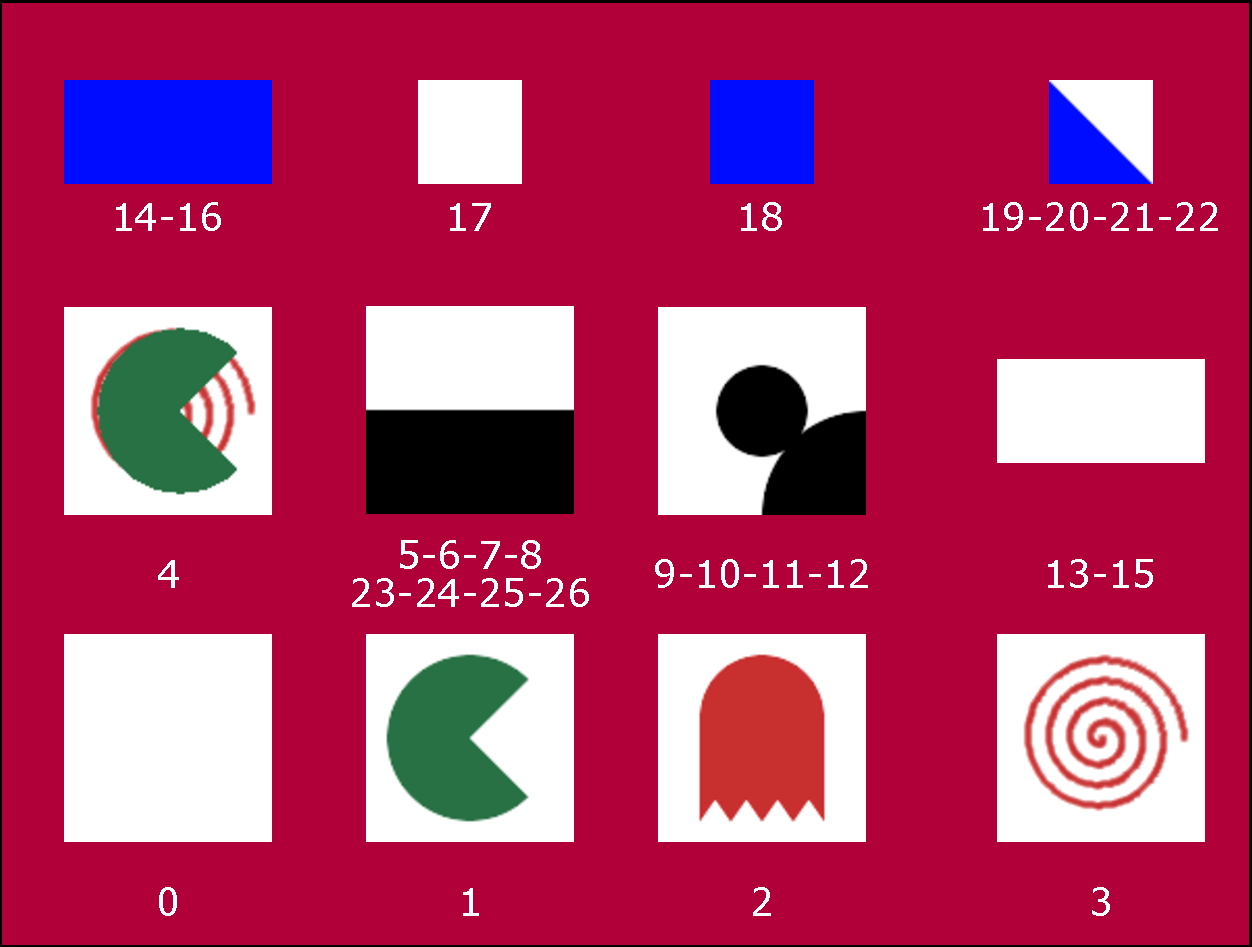
\includegraphics[width = .98\textwidth]{./4_Verifications/texture.pdf}
\caption{\label{fig:texture}Pack de texture utilisée}\vfill%
\end{minipage}\hfill%
\begin{minipage}{.48\textwidth}
\centering
\vfill%
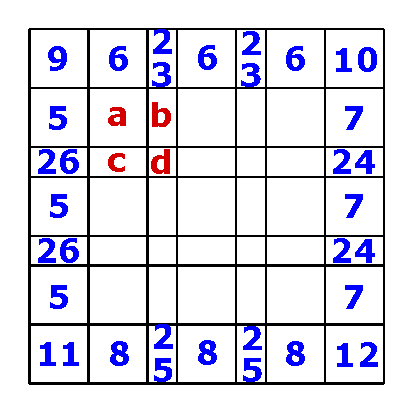
\includegraphics[width = .98\textwidth]{./4_Verifications/matriceTexture.pdf}
\caption{\label{fig:matTextu}Exemple de placement d'indice pour un labyrinthe 3x3.}\vfill%
\end{minipage}
\end{figure}
 Celles-ci sont organisées grâce à un ensemble d'indice, comme par exemple un labyrinthe 3x3, figure \ref{fig:matTextu}, où les indices en bleu sont statiques à tous les états du labyrinthe et où les indices en rouge, qui sont présents sur toutes cases similaires, sont susceptibles de changer. 
 \begin{description}
 \item[a] Les cases (indices $1$ à $4$).
 \item[b] Les murs verticaux (indices $16$ et $17$).
 \item[c] Les murs horizontaux (indices $15$ et $16$ ).
 \item[d] Les croisements (indices $17$ à $22$).
 \end{description}
 Dans une premier partie, nous plaçons les indices correspondant aux éléments a afficher dans une matrice et dans une seconde partie nous plaçons les images correspondantes dans un lot de trois matrices (pour les trois canaux de couleur RGB). Une troisième partie enregistre les matrices sous forme d'images et génère la vidéo.

 \section{Vérification Logicielle}
Les vérifications que nous avons effectuer son fait a partir du master daté du 30/01/2018. Si vous teste certaine validation maintenant elle ne fonctionnera plus vraiment en vu des modifications effectuer au cours du projet. 
\subsection{La case de sortie ne bouge pas}
Nous allons vérifier que la case de notre sortie du labyrinthe ne change pas de position pendant l'utilisation. Pour cela nous devons faire une analyse structurelle de notre code et une analyse de tous les cas possibles de notre case sortie. Pour faire l'analyse structurelle de notre code nous avons cherché tous les endroits du code où l'emplacement de la case sortie change. Notre analyse nous a donnée le document suivant:\\
\image{15cm}{4_Verifications/case_sortie.pdf}{Table des recherches de modification de l’emplacement de la case}
Nous avons aussi testé tous les cas possibles d'emplacement de notre sortie sur un labyrinthe 5x5 sans changé les murs. De ce test nous n'avons pas observé de problème.

\subsection{Fantôme et Pacman jamais sur la même case}
Pour tester que le fantôme et le Pacman ne sont jamais sur la même case nous avons fait un test "de pire cas possible" (on met des situations où on pense pourvoir faire apparaître ce bug s'il existe) sur différents labyrinthes. Pour cela nous avons placé plusieurs conditions initiales différentes, les tests sont faits avec un nombre de murs différents et plusieurs positions du fantôme et de Pacman différente. Pour nous retrouver dans les différentes situations nous avons fait le fichier excel suivant:\\


\image{18cm}{4_Verifications/pacman_ghost.pdf}{Excel de la vérification de Ghost et Pacman jamais sur la même case}
Des situations initiales suivantes nous avons lancé la première fonction de simulation qui permet de récupérer l'état du labyrinthe du début jusqu'à la fin de la simulation. Nous avons fait un oracle (c'est un programme qui va tourner en parallèle et qui nous permet de vérifier que les résultats obtenus par le code principale et le même que celui que l'on obtient par ce programme). Notre oracle va vérifier à chaque mouvement que la position de notre fantôme et du Pacman sont bien différentes.\\

Nous avons trouvé un bug lors de cette situation initiale : si les deux objets sont sur la même case à l'état initial, il n'y a aucun mouvement possible. Il faudrait vérifier les situations initiales dès le départ pour éviter ce cas qui devrait être impossible à arriver.\\

Les différents oracles que nous avons fait se trouvent dans le dossier validation2 qui se trouve dans le répertoire laby2player/validation.\\


\subsection{Les murs sont infranchissables}
Pour ce test nous nous somme placés dans deux situation différentes, l'une avec les murs qui ne bougent pas et l'autre avec les murs qui bougent. On a des situations initiale de murs différentes. Les différentes situations initiales sont récapitulées dans le fichier excel suivant:\\
\image{18cm}{4_Verifications/murs_infranchissables.pdf}{Résultats pour les murs sont infranchissables}
Pour vérifier que nos murs sont bien infranchissables dans notre oracle nous avons vérifié qu'à chaque déplacement du pacman ou du fantôme il n'y a pas de murs. On peut retrouver nos oracles dans le dossier validation3 dans le répertoire laby2player/validation.\\


\subsection{Les murs bougent dans la direction choisie}
Pour tester les murs qui bougent dans la direction choisie on s'est placé dans plusieurs situation différentes. Pour une situation donnée il faut obtenir les murs après un cycle. Quand on a les murs que l'on a obtenus et les murs que l'on a initialement on les compare.\\
On peut retrouver nos oracles dans le dossier validation4 dans répertoire laby2player/validation.\\
 

\subsection{Le programme s’arrête quand le pacman est sur la sortie}
Pour faire ce test nous avons utilisé plusieurs situations initiales différentes. Nous avons aussi dû faire ce test sur l'interface 1 joueur. On fait les situations suivantes :\\
\image{18cm}{4_Verifications/pacman_sortie.pdf}{Résultats pour "Le programme s’arrête quand le pacman est sur la sortie"}
%
On peut retrouver nos oracles dans le dossier validation7 dans le répertoire laby2player/validation.\\


\subsection{Le fantôme peut manger pacman}
Pour faire ces tests nous avons fait plusieurs situations initiales différentes :\\
\image{18cm}{4_Verifications/ghost_mange_pacman.pdf}{Exel des situations initiales}
Notre oracle va regarder si quand notre fantôme est à coté de notre pacman on a bien une incrémentation de notre compteur $caught$. Mais rapidement on s'est rendu compte qu'il y a un problème dans notre implémentation : quand les murs vont bouger alors que le fantôme et à coté du pacman le compteur s'incrémente. Il s'incrémente donc 2 fois : Une fois quand il se retrouvent à côté et une autre fois quand les murs se déplacent. Nous n'avons pas réussi encore a réglé ce problème. On peut retrouver nos oracles dans le dossier validation8 dans répertoire laby2player/validation.\\


\section{Validation formelle}\label{sec:validationFormelle}
%Validation formelle
%%%%%%%%%%%%%%%%%% J'ai modifié cette section pour y inclure les fonctions de génération de laby --Lucien
Pour la validation formelle nous avons créé plusieurs fonctions sur $Matlab$ qui nous permettent de générer le modèle de procédé du labyrinthe et les contraintes, le modèle de commande des mouvements des murs et en dernier lieu l'ordonnancement imposé (mouvement des murs puis mouvement des objets). Nous ne faisons que la modélisation 1 objet, la modélisation des 2 objets étant une des étapes restante à ce projet. Nous allons vous exposer dans cette partie l'ensemble des moyens que nous avons mis en place pour formaliser le labyrinthe.

\subsection{Génération des modèles} \label{subsec:generationModele}
\begin{center}
Nous allons dans cette subsection détaillé les fichiers qui se trouvent dans le dossier \emph{src/laby1player/automaton/modelGenerator}.
\end{center}
\subsubsection{Description des scripts} % la syllabe Scri est en répétition, vous pouvez changer ce titre. 
Vous trouverez dans le dossier spécifié un ensemble de fonctions qui permettent de générer plusieurs fichiers texte. Cette génération doit être lancée depuis le script principal qui porte le nom de : \underline{modelGenerator.m}. Il est possible de modifier les paramètres du labyrinthe dans ce script principal, en modifiant les variables \emph{wallsV}, \emph{wallsH}, \emph{pacman}, \emph{escape} et \emph{sched} qui sont respectivement la matrice des murs verticaux, des murs horizontaux, la position initiale du Pacman, la position (fixe) de la sortie et le séquencement qui sera appliqué.

Ce script principal fait ensuite appel à 3 fonctions : \emph{AutomatonStrutureLabyCreation}, \emph{AutomatonWallsContraintsCreation} et enfin \emph{AutomatonSchedulingCreation} qui vont se charger de créer les automates (vous trouverez une explication de chacun de ces automates dans le paragraphe décrivant les modèles). Ces fonctions renvoient des structures contenant l'ensemble des états et fonctions de transitions des automates qu'elles décrivent. Les structures sont en beaucoup de points ressemblantes à la classe AutomateGraph (\ref{parag:AutomateGraph}).


Enfin le script principal utilise les structures développées dans le paragraphe précédent pour en extraire les états/transitions de chaque automates. Il peut ensuite les écrire dans des fichiers textes (détaillés dans le paragraphe suivant) ou alors laisser les structures tel quel pour un e utilisation dans un autre script.

%%%% Fin des modifs -Lucien - Bisou :-)

\subsubsection{Description des modèles}\label{sub:descriptionDesModeles}
Tous les modèles créés par ces fonctions sont enregistrés sous format texte compatible avec $Desuma$ (\emph{SaveDesumaFile}). Par la suite on a importé ces fichiers dans $Desuma$ qui a créé les automates ($lab$, $walls$, $scheduling$) et dont nous nous sommes servi pour effectuer le produit parallèle entre les automates. Pour faire tourner ce code il faut allez dans répertoire modelGenerator et lancée le programme modelGenerator.m ce répertoire ce trouve dans src/laby1player/automaton.

Quand les modèles sont devenus trop lourds, nous avons chercher à implémenter le produit parallèle en \emph{Matlab} (voir plus de détail ci-dessous \ref{subsec:parallele}).
%ajoute rref.

On obtient bien une représentation automate de notre procédé, on va ensuite utiliser les outils de $Desuma$ pour vérifier les propriétés de notre labyrinthe et pouvoir effectuer des vérifications pour le valider.\\
On a remarqué que $Desuma$ ne nous affiche pas les états non accessibles, nous avons seulement les états accessibles et co-accessibles.
Par exemple si on prend le labyrinthe suivant:\\
\image{6cm}{4_Verifications/laby.pdf}{Labyrinthe 2x2}
De ce labyrinthe nous allons obtenir la modélisation du labyrinthe suivante (le fichier $lab$):\\
\image{6cm}{4_Verifications/baly2x2.JPG}{ modélisation du Labyrinthe 2x2}
Sur chaque état on indique quels sont les murs qu'il y a autour de cette case.\\
\\
\\

On obtient l'automate suivant pour l’ordonnancement (fichier $scheduling$):
\image{10cm}{4_Verifications/sched2x2.JPG}{ modélisation de l’ordonnancement du Labyrinthe 2x2}


On commence par les murs puis par les objets. On modélise tous les mouvements autorisés par rapport à la configuration des murs. On obtient un cycle des murs pour un labyrinthe on revient à la situation initiale des murs. Le cycle se trouve par 2 x dimension\_laby. On obtient la modélisation suivante (fichier $walls$):\\
\image{15cm}{4_Verifications/wall2x2.JPG}{modélisation de l’ordonnancement du Labyrinthe 2x2}
Sur chaque état on a les informations sur les murs autour et les déplacements autorisé.\\

\noindent\begin{tabularx}{\linewidth}{|c|c|X|}
%\begin{tabular}{|c|c|c|}
  \hline
  État & chemin non autorisé & remarques \\
  \hline
  1 & $L_1, D_1, U_1, R_2, D_2, L_3, D_3, U_3, D_4,R_4$  & On ne peut pas allez a gauche, bas et haut de la case 1. On ne peut pas allez a droit et haut de la case 2. On ne peut pas allez a gauche, bas et haut de la case 3. On ne peut pas allez a droit et bas de la case 4.  \\
  2 & $R_1, D_1, L_2, D_2, U_2, D_3,R_3 , L_4, D_4, U_4  $&  On ne peut pas allez a droit et haut de la case 1. On ne peut pas allez a gauche, bas et haut de la case 2. On ne peut pas allez a gauche, bas et haut de la case 3. On ne peut pas allez a droit et bas de la case 4.  \\
  3 & $R_1, D_1, L_2, D_2, U_2, D_3,R_3 , L_4, D_4, U_4$&  On ne peut pas allez a droit et haut de la case 1. On ne peut pas allez a gauche, bas et haut de la case 2. On ne peut pas allez a gauche, bas et haut de la case 3. On ne peut pas allez a droit et bas de la case 4.  \\
  4 & $L_1, D_1, U_1, R_2, D_2, L_3, D_3, U_3, D_4,R_4$  & On ne peut pas allez a gauche, bas et haut de la case 1. On ne peut pas allez a droit et haut de la case 2. On ne peut pas allez a gauche, bas et haut de la case 3. On ne peut pas allez a droit et bas de la case 4.  \\
  \hline
%\end{tabular}
\end{tabularx}\\


%Après avoir fait les 3 modélisations on fait le produit parallèle pour obtenir le procédé de notre labyrinthe avec toutes les dynamiques possibles de notre labyrinthe. On obtient une procédé avec des numéro pour chaque déplacement il faut donc faire un raffinement pour cela il faut enregistrer le fichier $Desuma$ de notre procédé sous forme $fsm$. Puis utiliser le programme rafineAutomaton.m qui ce trouve dans le répertoire modelGenerator qui ce trouve dans src/laby1player/automaton.\\

% Le fichier n'est pas à cet emplacment

%Quand on a notre procédé on va pouvoir faire le produit parallèle du procédé avec notre commande pour pacman. \\ % besoin de conclure un minimum ?

%On est arrivé à la conclusion que la commande mémoire n'est pas très efficace on trouve pas souvent la sortie. La commande avec priorité n'est pas très efficace nous plus mais on trouve plus facilement la sortie.\\ 
% Je veux pas sortir du Laby, le pacman oui par contre...
% 

%Mais rapidement on s'est rendu compte qu'avec le logiciel $Desuma$ nous avons des problèmes dû au nombre important de transitions et d'états. Nous avons donc décidé de passer par $Matlab$ pour faire notre produit parallèle.\\
% Automatisation nécessaire pour des raisons différentes à celle exprimés ici non ?


% Modif du paragraphe précédent Lucien
Après avoir fait les 3 modélisations nous faisons le produit parallèle pour obtenir le procédé de notre labyrinthe avec toutes les dynamiques possibles. Nous obtenons un procédé avec des numéros pour chaque déplacement : l'utilisation de ces numéros est nécessaire pour que les transitions ne soit pas confondu lors du calcul du produit parallèle. Cependant, ces numéros deviennent maintenant un problème, il faut donc faire un raffinement qui servira à enlever chaque numéro. Pour cela il faut enregistrer le fichier $Desuma$ de notre procédé sous forme $fsm$ (Fichier $\rightarrow $ Export $\rightarrow $ To UMDMES .fsm. Puis utiliser le programme \emph{rafineAutomaton.m} qui se trouve dans le répertoire \emph{src/laby1player/automaton/optimalCommand}.


Quand le procédé est construit, nous pouvons faire un produit parallèle avec notre commande pour Pacman. Nous obtenons ainsi l'ensemble des états qui sont atteignables par cette commande dans le labyrinthe étudié.


Nous sommes arrivés rapidement à la conclusion que la commande mémoire n'était pas très efficace, le pacman ne trouve pas souvent la sortie. La commande avec priorité n'est pas très efficace nous plus mais la sortie est atteinte plus facilement par le Pacman.


Mais rapidement nous avons eu des problèmes avec le logiciel $Desuma$ dû au nombre important de transitions et d'états ainsi qu'à cause de la redondance de l'exercice (Ouvrir des fichiers, Copier - Coller, exporter...). Nous avons donc décidé de passer par $Matlab$ pour faire notre produit parallèle et automatiser entièrement ce qui vient d'être décrit dans cette partie (\ref{subsec:parallele}). Cependant, nous avons créer un sript dans un premier temps qui permet d'utiliser l'automate généré dans cette subsection pour en déterminer le(s) chemins (s'il existent) qui mène le Pacman vers la sortie. % ... -- Review Lucien
Ce sujet sera l'objet  de notre prochain sous-section.
\subsection{Déterminer l'ensemble des chemins}\label{sub:ensembleDesChemins}% Need a Fucking better title !! TODO
% Un chemin pour aller vers le far Ouest
% L'autre pour aller à l'OuNERA
% L'autre pour aller vers Madrid
\begin{center}
L'ensemble des scripts décrit ici sont disponibles dans \emph{src/laby1player/automaton/optimalCommand}.
\end{center}

Dans le cas où l'automate obtenu après la composition parralèle possède toujours 1 (ou plusieurs) état(s) marqué(s), nous avons souhaité été capable de déterminé, de manière générique, quels était les séquence amenant à ces états marqués depuis l'état initial. Pour cela, nous avons fait appel à une librairie \emph{Matlab} : \emph{graph}. Cet ensemble de fonction utilise des algorithmes issus de la résolution de Bellman-Ford pour calculer, à partir d'un graph, l'ensemble des chemins possibles, en les clasant du plus court au plus long.

Pour adapter cette fonction à notre automate, nous avons été obligé de transposer l'automate en un graph. C'est l'objet de la fonction \emph{optimalCommand} disponible dans le fichier \emph{.m} qui porte son nom. Cette fonction prend en entrée l'ensemble des matrices de transition qui permettent de décrire les transitions de l'automate, l'état de départ et l'état d'arrivé de l'algorithme. Elle associe un poid équivalent à chaque transition et supprime les transitions stables (elles ne sont pas acceptées par l'algorithme). La fonction affiche ensuite tout les chemins qui ont été trouvé par l'algorithme, du plus court au plus long. 

Pour permettre son utilisation directe avec l'automate calculé via \emph{DESUMA} dans \ref{sub:descriptionDesModeles}, nous avons crée un script principal \emph{main}. ce programme va récupérer les données depuis un fichier \emph{DESUMA}, en extraire les matrices de transitions pour les envoyer ensuite vers \emph{optimalCommand}. 


\paragraph*{Remarque} Pour l'utiliser avec un procédé, vous devez modifier le nom appelé dans la ligne 17. Veuillez faire attention aux noms utilisé aux transitions dans l'automate que vous appelé : ils doievent avoir le même nom que dans la liste instancié à l ligne 16.

\subsection{Automatisation de la composition parallèle avec Matlab}
\label{subsec:parallele}
Par soucis de simplification, nous avons choisi d'effectuer le calcul du produit parallèle avec $Matlab$. Il nous a donc été nécessaire de créer un ensemble de classe et fonction pour pouvoir jouir de cette possibilité. Nous allons vous les présenter dans cette sous-section. Dans un premier temps, nous allons vous expliquer comment nous avons mis en œuvre le calcul du produit parallèle. Ensuite, nous expliquerons la classe \emph{AutomateGraph}, classe qui modélise un automate et le retranscrit en \emph{Matlab}. Enfin, nous vous présenterons le script général qui permet de lancer toute l'exécution. 

\paragraph*{Produit Parallèle}
La composition parallèle est un outil très utilisé dans la théorie des automates. Nous l'utilisions dans un premier temps avec le logiciel \emph{DESUMA} mais nous souhaitons maintenant automatiser ce calcul. Pour cela, nous avons développé l'algorithme de la manière suivante :
Soit un premier automate $ A1$  avec un langage $L_{A1}$  et un ensemble de matrice de transition : $M_{A1}$.
Soit un second automate $A2$  avec un langage $L_{A2}$  et un ensemble de matrice de transition : $M_{A2}$.\\
Nous avons l'automate $A$ qui est le produit parallèle de $A1$ et de $A2$  qui s'écrit :
\begin{align*}
& A = A1 \sslash A2\\
&L_A = L_{A1} \bigcup L_{A2} \text{ avec } L_A\text{ Langage de A}\\
\end{align*}
Pour l'ensemble des matrices de $A$, nous devons procéder de la sorte : pour chaque événements communs aux deux automates, alors :
\begin{equation}
M_{A} = M_{A1} \otimes M_{A2}
\end{equation}
Sinon, pour chaque événements de A1 (qui n'est pas inclus dans $L_{A2}$) :
\begin{equation}
M_{A} = M_{A1} \otimes 1\!\!1 
\end{equation}
Sinon pour chaque événements de A2 (qui n'est pas inclus dans $L_{A1}$) :
\begin{equation}
M_{A} = 1\!\!1 \otimes M_{A2}
\end{equation}
La fonction $Matlab$ développée est disponible dans src/laby1player/automaton/ParrallelComposition.m. 

\paragraph*{Classe Automate déterministe : AutomateGraph}\label{parag:AutomateGraph}
L'objectif de cette classe $Matlab$ est de permettre une utilisation des outils développés pour la validation formelle du labyrinthe. Elle est composé de 4 attributs sous forme de structure : "state", "transition", "matrixTrans", "langage" et "vector", les détails de chaque attributs est disponible dans le code source de la classe (fichier AutomateGraph.m dans le dossier : src/laby\_1\_player/automaton). Chaque objet $AutomateGraph$ peut accéder à une liste de méthodes qui vont permettre en autre de modifier son langage, d'effectuer des passages entre des description différente, tel que la transformation d'une description vectorielle à matricielle, ou encore d'une description Etats/Transition vers une description en matrice.


Il existe aussi des méthodes plus complexes : la méthode \underline{PathResearche} est une fonction qui va permettre de trouver l'ensemble des chemins menant d'un état de départ à un état d'arrivé. -Donc, pour obtenir le langage marqué, il suffit de placé l'état initial et l'état marqué respectivement) Une dernière méthode \underline{sortStateAutomate} permet d’éliminer les états inaccessible de l'automate, en parcourant chaque transition. De plus ample explication sont disponibles dans le fichier présenté au début de ce paragraphe.  



\paragraph*{Utilisation avec un script complet}
Pour pouvoir exécuter la vérification d'un objectif avec $Matlab$, vous pouvez utiliser le script $MainLaby.m$, disponible dans src/laby1player/automaton/. Ce script va automatiquement généré un procédé grâce aux scripts utilisés dans le début de cette section et lancé depuis ModelGenerator.m. (Si vous souhaitez modifier le labyrinthe, veuillez-vous référer à la documentation du code source) Une fois les modèles obtenus, il les enregistre sous forme d'un objet appartenant à la classe $AutomateGraph$. Le script effectue ensuite automatiquement un produit parallèle pour obtenir le modèle de procédé complet. 

Il vous demande ensuite de choisir avec quel objectif vous voulez composez le modèle de commande. Le script s'occupe ensuite d'établir ce modèle avec un dernier produit parallèle.  


